\documentclass{ximera}

 

\usepackage{epsfig}

\graphicspath{
  {./}
  {figures/}
}

\usepackage{morewrites}
\makeatletter
\newcommand\subfile[1]{%
\renewcommand{\input}[1]{}%
\begingroup\skip@preamble\otherinput{#1}\endgroup\par\vspace{\topsep}
\let\input\otherinput}
\makeatother

\newcommand{\includeexercises}{\directlua{dofile("/home/jim/linearAlgebra/laode/exercises.lua")}}

%\newcounter{ccounter}
%\setcounter{ccounter}{1}
%\newcommand{\Chapter}[1]{\setcounter{chapter}{\arabic{ccounter}}\chapter{#1}\addtocounter{ccounter}{1}}

%\newcommand{\section}[1]{\section{#1}\setcounter{thm}{0}\setcounter{equation}{0}}

%\renewcommand{\theequation}{\arabic{chapter}.\arabic{section}.\arabic{equation}}
%\renewcommand{\thefigure}{\arabic{chapter}.\arabic{figure}}
%\renewcommand{\thetable}{\arabic{chapter}.\arabic{table}}

%\newcommand{\Sec}[2]{\section{#1}\markright{\arabic{ccounter}.\arabic{section}.#2}\setcounter{equation}{0}\setcounter{thm}{0}\setcounter{figure}{0}}

\newcommand{\Sec}[2]{\section{#1}}

\setcounter{secnumdepth}{2}
%\setcounter{secnumdepth}{1} 

%\newcounter{THM}
%\renewcommand{\theTHM}{\arabic{chapter}.\arabic{section}}

\newcommand{\trademark}{{R\!\!\!\!\!\bigcirc}}
%\newtheorem{exercise}{}

\newcommand{\dfield}{{\sf dfield9}}
\newcommand{\pplane}{{\sf pplane9}}

\newcommand{\EXER}{\section*{Exercises}}%\vspace*{0.2in}\hrule\small\setcounter{exercise}{0}}
\newcommand{\CEXER}{}%\vspace{0.08in}\begin{center}Computer Exercises\end{center}}
\newcommand{\TEXER}{} %\vspace{0.08in}\begin{center}Hand Exercises\end{center}}
\newcommand{\AEXER}{} %\vspace{0.08in}\begin{center}Hand Exercises\end{center}}

% BADBAD: \newcommand{\Bbb}{\bf}

\newcommand{\R}{\mbox{$\Bbb{R}$}}
\newcommand{\C}{\mbox{$\Bbb{C}$}}
\newcommand{\Z}{\mbox{$\Bbb{Z}$}}
\newcommand{\N}{\mbox{$\Bbb{N}$}}
\newcommand{\D}{\mbox{{\bf D}}}
\usepackage{amssymb}
%\newcommand{\qed}{\hfill\mbox{\raggedright$\square$} \vspace{1ex}}
%\newcommand{\proof}{\noindent {\bf Proof:} \hspace{0.1in}}

\newcommand{\setmin}{\;\mbox{--}\;}
\newcommand{\Matlab}{{M\small{AT\-LAB}} }
\newcommand{\Matlabp}{{M\small{AT\-LAB}}}
\newcommand{\computer}{\Matlab Instructions}
\newcommand{\half}{\mbox{$\frac{1}{2}$}}
\newcommand{\compose}{\raisebox{.15ex}{\mbox{{\scriptsize$\circ$}}}}
\newcommand{\AND}{\quad\mbox{and}\quad}
\newcommand{\vect}[2]{\left(\begin{array}{c} #1_1 \\ \vdots \\
 #1_{#2}\end{array}\right)}
\newcommand{\mattwo}[4]{\left(\begin{array}{rr} #1 & #2\\ #3
&#4\end{array}\right)}
\newcommand{\mattwoc}[4]{\left(\begin{array}{cc} #1 & #2\\ #3
&#4\end{array}\right)}
\newcommand{\vectwo}[2]{\left(\begin{array}{r} #1 \\ #2\end{array}\right)}
\newcommand{\vectwoc}[2]{\left(\begin{array}{c} #1 \\ #2\end{array}\right)}

\newcommand{\ignore}[1]{}


\newcommand{\inv}{^{-1}}
\newcommand{\CC}{{\cal C}}
\newcommand{\CCone}{\CC^1}
\newcommand{\Span}{{\rm span}}
\newcommand{\rank}{{\rm rank}}
\newcommand{\trace}{{\rm tr}}
\newcommand{\RE}{{\rm Re}}
\newcommand{\IM}{{\rm Im}}
\newcommand{\nulls}{{\rm null\;space}}

\newcommand{\dps}{\displaystyle}
\newcommand{\arraystart}{\renewcommand{\arraystretch}{1.8}}
\newcommand{\arrayfinish}{\renewcommand{\arraystretch}{1.2}}
\newcommand{\Start}[1]{\vspace{0.08in}\noindent {\bf Section~\ref{#1}}}
\newcommand{\exer}[1]{\noindent {\bf \ref{#1}}}
\newcommand{\ans}{}
\newcommand{\matthree}[9]{\left(\begin{array}{rrr} #1 & #2 & #3 \\ #4 & #5 & #6
\\ #7 & #8 & #9\end{array}\right)}
\newcommand{\cvectwo}[2]{\left(\begin{array}{c} #1 \\ #2\end{array}\right)}
\newcommand{\cmatthree}[9]{\left(\begin{array}{ccc} #1 & #2 & #3 \\ #4 & #5 &
#6 \\ #7 & #8 & #9\end{array}\right)}
\newcommand{\vecthree}[3]{\left(\begin{array}{r} #1 \\ #2 \\
#3\end{array}\right)}
\newcommand{\cvecthree}[3]{\left(\begin{array}{c} #1 \\ #2 \\
#3\end{array}\right)}
\newcommand{\cmattwo}[4]{\left(\begin{array}{cc} #1 & #2\\ #3
&#4\end{array}\right)}

\newcommand{\Matrix}[1]{\ensuremath{\left(\begin{array}{rrrrrrrrrrrrrrrrrr} #1 \end{array}\right)}}

\newcommand{\Matrixc}[1]{\ensuremath{\left(\begin{array}{cccccccccccc} #1 \end{array}\right)}}



\renewcommand{\labelenumi}{\theenumi)}
\newenvironment{enumeratea}%
{\begingroup
 \renewcommand{\theenumi}{\alph{enumi}}
 \renewcommand{\labelenumi}{(\theenumi)}
 \begin{enumerate}}
 {\end{enumerate}\endgroup}



\newcounter{help}
\renewcommand{\thehelp}{\thesection.\arabic{equation}}

%\newenvironment{equation*}%
%{\renewcommand\endequation{\eqno (\theequation)* $$}%
%   \begin{equation}}%
%   {\end{equation}\renewcommand\endequation{\eqno \@eqnnum
%$$\global\@ignoretrue}}

%\input{psfig.tex}

\author{Martin Golubitsky and Michael Dellnitz}

%\newenvironment{matlabEquation}%
%{\renewcommand\endequation{\eqno (\theequation*) $$}%
%   \begin{equation}}%
%   {\end{equation}\renewcommand\endequation{\eqno \@eqnnum
% $$\global\@ignoretrue}}

\newcommand{\soln}{\textbf{Solution:} }
\newcommand{\exercap}[1]{\centerline{Figure~\ref{#1}}}
\newcommand{\exercaptwo}[1]{\centerline{Figure~\ref{#1}a\hspace{2.1in}
Figure~\ref{#1}b}}
\newcommand{\exercapthree}[1]{\centerline{Figure~\ref{#1}a\hspace{1.2in}
Figure~\ref{#1}b\hspace{1.2in}Figure~\ref{#1}c}}
\newcommand{\para}{\hspace{0.4in}}

\renewenvironment{solution}{\suppress}{\endsuppress}

\ifxake
\newenvironment{matlabEquation}{\begin{equation}}{\end{equation}}
\else
\newenvironment{matlabEquation}%
{\let\oldtheequation\theequation\renewcommand{\theequation}{\oldtheequation*}\begin{equation}}%
  {\end{equation}\let\theequation\oldtheequation}
\fi

\makeatother


\title{Stylized Phase Portraits}

\begin{document}
\begin{abstract}
\end{abstract}
\maketitle

  \label{S:SPP}
\index{stylized phase portrait}\index{phase!portrait!stylized}


In Section~\ref{S:linearization} we discussed phase portraits of systems with 
equilibria but without periodic solutions.  In Section~\ref{S:periodic} we 
discussed briefly certain planar systems having limit cycles.  In this 
section we combine the discussions on equilibria and periodic solutions; 
together these discussions allow us to give a strategy for determining 
numerically the phase portraits of a broad class of planar autonomous 
differential equations --- the Morse-Smale differential equations.
 
Planar phase portraits indicate all equilibria, periodic
solutions, and connecting trajectories.  The simplest phase
portraits are those that describe the dynamics of differential
equations satisfying the following assumptions: \index{hyperbolic}
\begin{itemize}
\item	All equilibria are hyperbolic.
\item	All periodic solutions are limit cycles.
\item	There are no trajectories connecting two saddle points.
\end{itemize}
A planar system of differential equations that satisfies these
three conditions is called a {\em Morse-Smale\/} system.  
\index{Morse-Smale system}

\begin{definition} \label{D:stylized}
A {\em stylized phase portrait\/} of a planar autonomous system
of differential equations is a picture illustrating all
equilibria and their type, all limit cycles, and all connecting
trajectories.
\end{definition}\index{stylized phase portrait}\index{phase!portrait!stylized}

Generally, it is not an easy task to draw the stylized phase
portrait of a differential equation.  However, using {\sf pplane8\/} 
we can attempt to draw the phase portrait of a
Morse-Smale system on a given rectangle in the following way.
\begin{enumerate}
\item Using both analysis and numerics, find the equilibria of
the differential equation.
\item Mark these equilibria and their type.  
\item Draw the stable and unstable orbits of saddles.  
\index{saddle!stable and unstable orbits}
\item Determine the number and stability of limit cycles.  
\end{enumerate}
Putting this information together allows us to draw planar phase
portraits.

\subsection*{The {\sf pplane8} Default Equation}

As an example, we discuss the stylized phase portrait of the 
{\sf pplane8}\index{\computer!pplane8} default equation:
\begin{equation}  \label{e:default}
\begin{array}{rcl}
\dot{x} & = & 2x-y+3(x^2-y^2)+2xy \\
\dot{y} & = & x-3y-3(x^2-y^2)+3xy
\end{array}
\end{equation} 
Our goal is to draw the stylized phase portrait of this system
of differential equations on some rectangle in the plane, and we
choose the default rectangle: $-2\leq x\leq 4$, $-4\leq y\leq 2$.

Inspection of \eqref{e:default} shows that the origin\index{origin} 
is an equilibrium.  By clicking on the {\sf Find an equilibrium point}
button, we see that the origin is a saddle.  By clicking on the
{\sf plot stable and unstable orbits} button and then clicking
on the mouse when the cross hairs are near the origin, {\sf
pplane8} plots the stable and unstable orbits of this saddle.
See Figure~\ref{F:default0}.

\begin{figure}[htb]
           \centerline{%
	   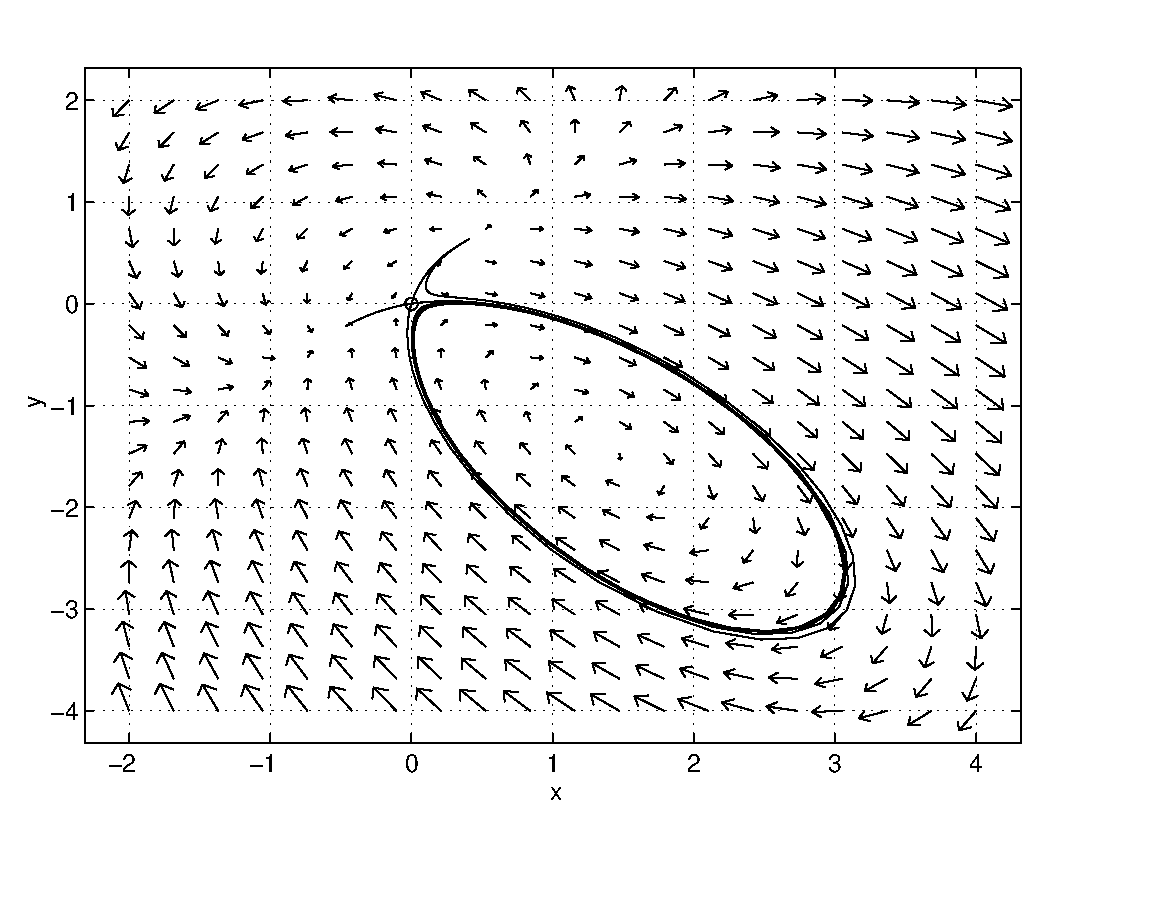
\psfig{file=../figures/default0.eps,width=3.2in}
	   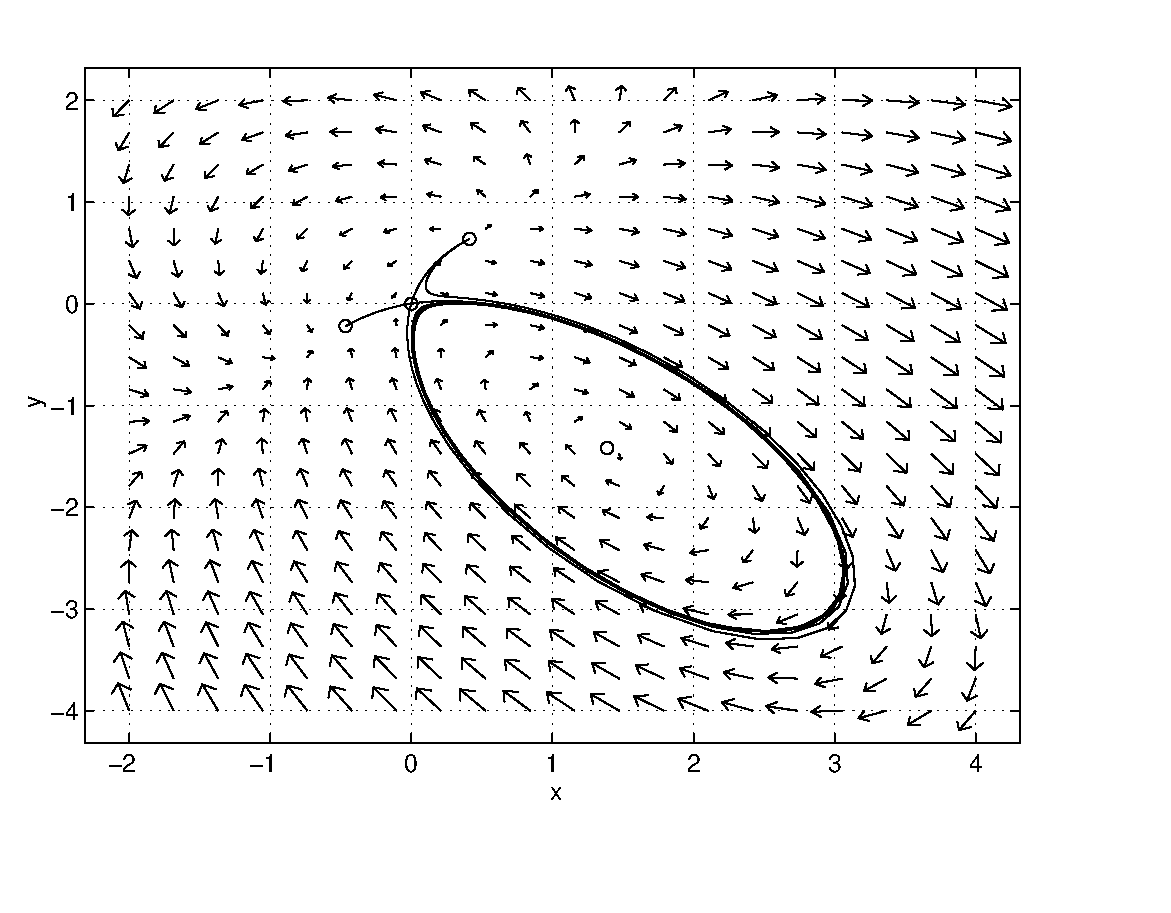
\psfig{file=../figures/default1.eps,width=3.2in}}
           \caption{(Left) Stable and unstable orbits of the saddle at
		the origin in \protect\eqref{e:default}. (Right) Picture 
		of \protect\eqref{e:default} with equilibria added.}
           \label{F:default0}
\end{figure}
 
This calculation reveals several interesting features in the
phase portrait of \eqref{e:default}.  First, both stable orbits limit on the 
same equilibrium, and that equilibrium is near $(0.5,0.5)$.  Second, one 
unstable orbit limits on an equilibrium near $(-0.5,-0.2)$, while the other 
unstable orbit limits on what appears to be a limit cycle.  It follows from 
Theorem~\ref{T:PB} that there must be an equilibrium inside this limit cycle 
--- probably near $(1.3,-1.3)$.  Using the information and the {\sf
Find an equilibrium point} button, we can locate three
equilibria:
\begin{itemize}
\item	A nodal sink at $(-0.4661,-0.2209)$,
\item	A nodal source at $(0.4125,0.6386)$,
\item	A spiral source at $(1.387,-1.418)$. 
\end{itemize}
Entering these equilibria yields the phase portrait in 
Figure~\ref{F:default0} (right). 

We now draw the stylized phase portrait\index{stylized phase portrait}
\index{phase!portrait!stylized} for \eqref{e:default},
indicating the four equilibria and their type, the periodic
solutions, and the connecting trajectories. See
Figure~\ref{F:default2} (right).  A picture with additional 
trajectories is shown on the left of that figure.

\begin{figure}[htb]
           \centerline{%
	   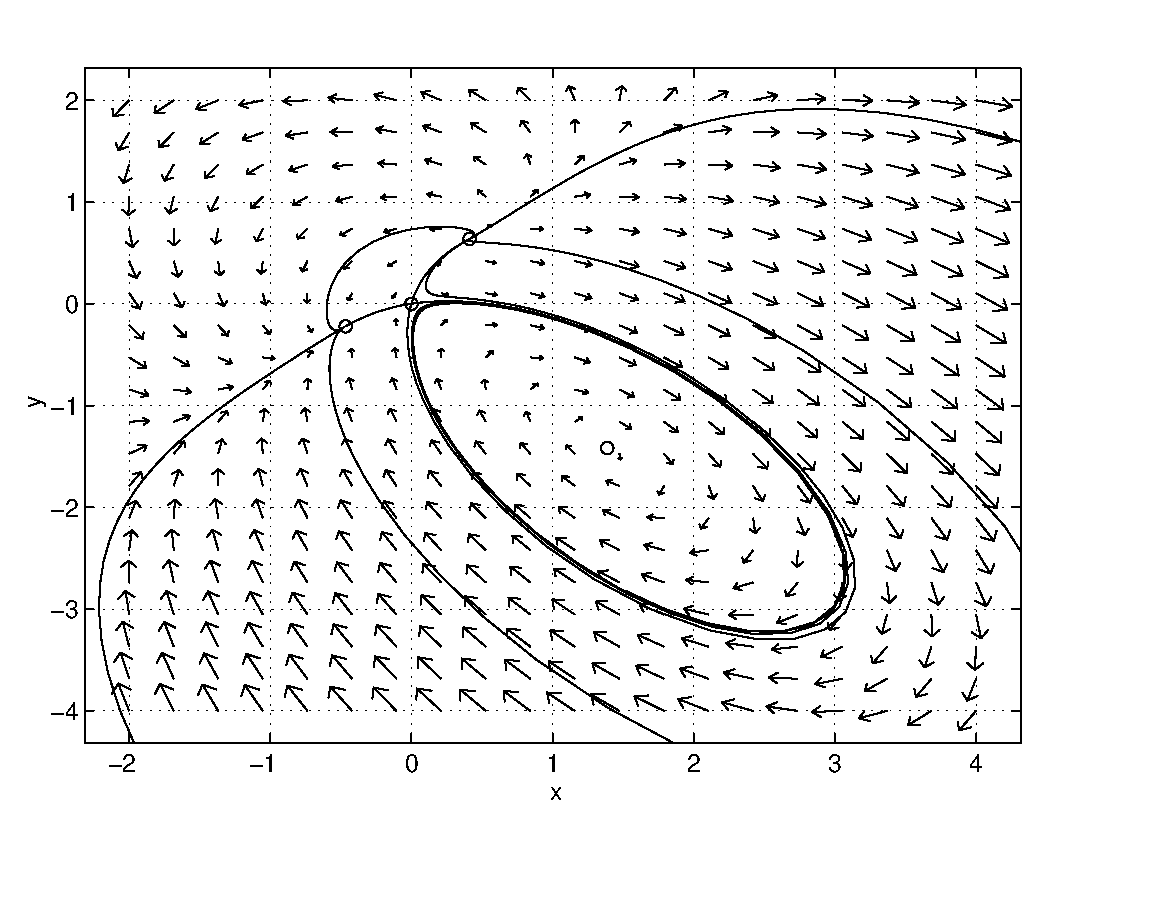
\psfig{file=../figures/default2.eps,width=3.0in}
	   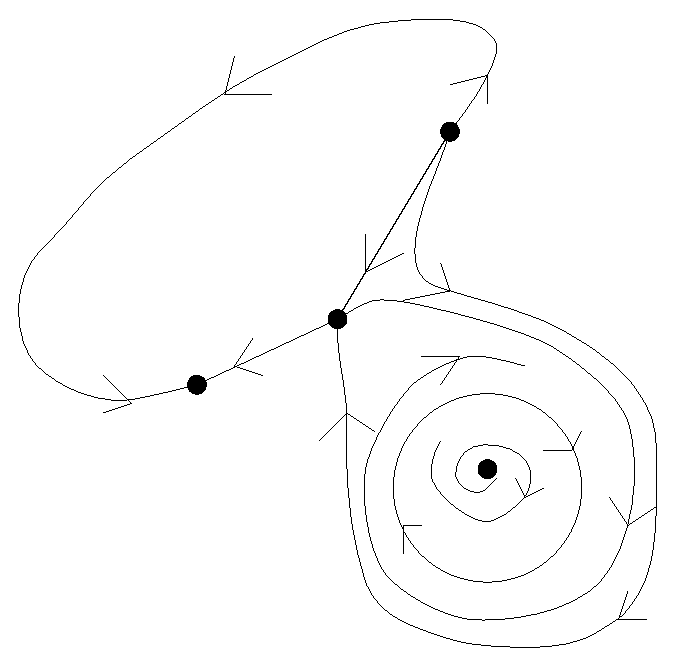
\psfig{file=../figures/default4.eps,height=2.2in}
		}
           \caption{(Left) Additional trajectories of 
\protect\eqref{e:default}. (Right) Stylized phase portrait
indicating equilibria, periodic solutions and connecting trajectories.}
           \label{F:default2}
\end{figure}

It is reasonable to wonder whether this somewhat ad hoc process
for finding the stylized phase portrait will always work.  The
simple answer is {\em no} --- but much progress can be made if
one proceeds cautiously.  

For example, one numerical difficulty appears in the analysis of
the default system \eqref{e:default}.  Clicking inside the limit
cycle, shows a trajectory that spirals to a limit cycle in
forward time, as expected. In backward time, however, the
trajectory spirals towards the spiral source --- but never makes
it --- and {\sf pplane8} indicates the possible existence of a
second periodic solution.  In fact, no such periodic solution
exists. This point can be clarified using the zoom feature near
the spiral source.  These numerical calculations verify that the 
default system \eqref{e:default} is Morse-Smale.

\EXER

\CEXER

\begin{exercise} \label{c8.4.1}
Use {\sf pplane8} to determine the stylized phase portrait for 
the system
\begin{matlabEquation}\label{phaseportrait1}
\begin{array}{rcl}
\dot{x} & = &  2x-y+3\cos(x+y)  \\
\dot{y} & = &  x -3y -2xy
\end{array}
\end{matlabEquation}
on the square $-10 \leq x,y \leq 10$.  Indicate all equilibria
(and their types) and all periodic solutions.

\begin{solution}

Graph the system using {\tt pplane5}.  Then, find a saddle point at
$(-0.7426,-0.4902)$.  Plot the unstable and stable orbits.  The unstable
orbits and one stable orbit leave the graph window.  The other stable
orbit limits on a periodic solution around another equilibrium, the
spiral sink at $(-1.298,-3.209)$.  These are the only equilibria of
the system in this region.  The phase portrait is shown in
Figure~\ref{c8.4.1}.

\begin{figure}[htb]
                       \centerline{%
                       \psfig{file=exfigure/8-4-1.eps,width=3.0in}}
                \exercap{c8.4.1}
\end{figure}

\end{solution}
\end{exercise}  

\begin{exercise} \label{c8.4.2}
Use {\sf pplane8} to determine the number of equilibria and their
types for the system
\begin{matlabEquation}\label{MATLAB:2}
\begin{array}{rcl}
\dot{x} & = &  2x-y+3\cos(x+y)  \\
\dot{y} & = &  x -y -2\sin(x-y)
\end{array}
\end{matlabEquation}
in the rectangle $-2 \leq x \leq 4$, $-3 \leq y \leq 6$.  

\begin{solution}

Use {\tt pplane5} to graph the system and find equilibria.  The
command {\tt List computed equilibrium points} yields:
\begin{verbatim}
(-0.6724, -0.6724)      Nodal source.
(1.4782, 3.3737)        Saddle point.
(1.9929, 1.9929)        Nodal source.
(-0.6778, 1.2177)       Spiral sink.
(-1.0464, 0.8491)       Saddle point.
(-0.1485, -2.0440)      Saddle point.
(4.1299, 6.0254)        Saddle point.
(3.2051, 5.1006)        Spiral sink.
(-2.8222, -4.7177)      Saddle point.
(-1.3103, -3.2058)      Spiral sink.
\end{verbatim}
Figure~\ref{c8.4.2} shows a {\tt pplane5} graph of the system.

\begin{figure}[htb]
                       \centerline{%
                       \psfig{file=exfigure/8-4-2.eps,width=3.0in}}
                \exercap{c8.4.2}
\end{figure}

\end{solution}
\end{exercise}  

\begin{exercise} \label{c8.4.3}
Use {\sf pplane8} to determine the number of equilibria and their types, the
number of limit cycles, and the connecting trajectories for the system
\begin{matlabEquation}\label{MATLAB:3}
\begin{array}{rcl}
\dot{x} & = & 2-y^2-((x^2-2)^2+(y^2-2)^2-1)(x^2-2)-0.2x  \\
\dot{y} & = & x^2-2-((x^2-2)^2+(y^2-2)^2-1)(y^2-2)
\end{array}
\end{matlabEquation}
in the square $-3 \leq x,y \leq 3$.   
\begin{itemize}
\item[(a)] Draw a qualitative phase portrait for this system.  
\item[(b)] Characterize all solutions to this differential equation that 
stay within the square $-3 \leq x,y \leq 3$ for all forward and backward time 
$t$.
\item[(c)] Draw the time series in $x$ versus $t$ for the trajectory whose
initial condition is $(0,0)$.
\end{itemize}

\begin{solution}

The equilibria and their types are:
\begin{verbatim}
(1.4650, 1.3590)        Spiral source.           
(-1.3651, -1.4635)      Spiral sink.             
(1.4650, -1.3590)       Saddle point.            
(-1.3651, 1.4635)       Saddle point. 
\end{verbatim}
There are two limit cycles: one surrounding the spiral source at
$(1.4650, 1.3590)$ and one surrounding the spiral sink at $(-1.3651, -1.4635)$.

(a) A graph of the system is shown in Figure~\ref{c8.4.3}a.

(b) The four equilibria surround a roughly rectangular region.  As shown
by the connecting trajectories in the graph, all trajectories with
initial points inside this region remain in this region.  Note that this
includes trajectories with initial conditions inside the limit cycles.
All trajectories outside this region leave the window
$-3 \leq x,y \leq 3$ in forward or backward time.

(c) The {\tt pplane5} time series for the solution starting at $(0,0)$ is
shown in Figure~\ref{c8.4.3}b.

\begin{figure}[htb]
                       \centerline{%
                       \psfig{file=exfigure/8-4-3a.eps,width=2.75in}
                       \psfig{file=exfigure/8-4-3b.eps,width=2.75in}}
                \exercaptwo{c8.4.3}
\end{figure}

\end{solution}
\end{exercise}  

\begin{exercise} \label{c8.4.4}
Draw the stylized phase portrait of \eqref{8.3.3eq}.

\begin{solution}
See the figure for Exercise~\ref{c8.3.3} in
Section~\ref{S:periodic}.

\end{solution}
\end{exercise}

\noindent In Exercises~\ref{c8.4.5a} -- \ref{c8.4.5b} answer the following 
four questions for the given system of differential equations:
\begin{itemize}
\item[(a)]  How many equilibria does the system of differential equations 
have?  Any equilibrium that you find using {\sf pplane8} may be considered an 
actual equilibrium.  But use analysis to prove that you have found them all.
\item[(b)]  How many limit cycles does the system of differential equations 
have?  Base your answer on numerical exploration using {\sf pplane8}.
\item[(c)]  By hand (and not necessarily to scale) sketch the phase portrait.
\item[(d)]  Indicate which initial conditions have solutions that stay
bounded in forward time.
\end{itemize}
\begin{exercise}  \label{c8.4.5a}
\begin{matlabEquation}\label{MATLAB:4}
\begin{array}{rcl}
\dot{x} & = & 0.04x - y - 3y^2 + 2.5xy\\
\dot{y} & = & x - 3x^2 + 2x^2y.
\end{array}
\end{matlabEquation}

\begin{solution}

\ans There are five equilibria and two limit cycles.  The phase portrait is
given in Figure~\ref{c8.4.5a}a.  The orbits that stay bounded in
forward time are indicated in Figure~\ref{c8.4.5a}b.

\soln (a)  Using {\sf pplane5} we can find five equilibria
\begin{verbatim}
(0.0000, 0.0000)        Spiral source.           
(1.8519, 1.2300)        Nodal source.            
(0.3445, 0.0485)        Saddle point.            
(0.3102, -0.1118)       Spiral sink.             
(0.0000, -0.3333)       Saddle point.            
\end{verbatim}
We can show that there are at most five equilibria by solving:
\begin{eqnarray*}
0.04x - y - 3y^2 + 2.5xy & = & 0\\
x - 3x^2 + 2x^2y & = & 0.
\end{eqnarray*}  
Factoring the second equation leads to 
\[
x=0 \quad \mbox{ or } \quad x = \frac{1}{3-2y}.
\]
Substituting $x=0$ into the first equation leads to the equilibria
$(0,0)$ and $(0,-\frac{1}{3})$. Substituting $x = \frac{1}{3-2y}$ into the
first equation yields
\[
\frac{0.04+2.5y}{3-2y} -(y+3y^2)=0.
\]
Multiplying this equation by $3-2y$ leads to a cubic equation that has at most
three roots.  Thus there are at most five equilibria in this system of
differential equations.

\noindent (b) There is numerical evidence for two limit cycles
one surrounding the spiral source at the origin and one surrounding the
spiral sink at $(0.3102, -0.1118)$.

\noindent (c)  The five equilibria, two limit cycles, and the stable and
unstable orbits of saddles are shown in Figure~\ref{c8.4.5a}a.

\noindent (d)  The solutions that stay bounded in forward time include the
equilibria, limit cycle and those indicated in Figure~\ref{c8.4.5a}b.

\begin{figure}[htb]
                       \centerline{%
                        \psfig{file=exfigure/8-4-5a.eps,width=2.75in}
			\psfig{file=exfigure/8-4-5a2.eps,width=2.75in}}
                \exercaptwo{c8.4.5a}
\end{figure}




\end{solution}
\end{exercise}
\begin{exercise}  \label{c8.4.5b}
\begin{matlabEquation}\label{MATLAB:5}
\begin{array}{rcl}
\dot{x} & = & 0.05x - y - 3y^2 + 2xy \\
\dot{y} & = & x - 3x^2 + x^2y.
\end{array}
\end{matlabEquation}

\begin{solution}

\ans There are five equilibria and one limit cycle.  The phase portrait is
given in Figure~\ref{c8.4.5b}a.  The orbits that stay bounded in forward time
are indicated in Figure~\ref{c8.4.5b}b.

\soln  (a)  Using {\sf pplane5} we can find five equilibria
\begin{verbatim}
(0.0000, 0.0000)        Spiral source.           
(4.6347, 2.7842)        Nodal source.            
(0.3377, 0.0384)        Saddle point.            
(0.3169, -0.1560)       Spiral sink.             
(0.0000, -0.3333)       Saddle point.            
\end{verbatim}
We can show that there are at most five equilibria by solving:
\begin{eqnarray*}
0.05x - y - 3y^2 + 2xy & = & 0\\
x - 3x^2 + x^2y & = & 0.
\end{eqnarray*}  
Factoring the second equation leads to 
\[
x=0 \quad \mbox{ or } \quad x = \frac{1}{3-y}.
\]
Substituting $x=0$ into the first equation leads to the equilibria
$(0,0)$ and $(0,-\frac{1}{3})$. Substituting $x = \frac{1}{3-y}$ into the
first equation yields
\[
\frac{0.05+2y}{3-y} -(y+3y^2)=0.
\]
Multiplying this equation by $3-y$ leads to a cubic equation that has at most
three roots.  Thus there are at most five equilibria in this system of
differential equations.

\noindent (b) There is numerical evidence for just one limit cycle
surrounding the equilibrium at the origin.

\noindent (c)  The five equilibria, one limit cycle, and the stable and
unstable orbits of saddles are shown in Figure~\ref{c8.4.5b}a.

\noindent (d)  The solutions that stay bounded in forward time include the
equilibria, limit cycle and those indicated in Figure~\ref{c8.4.5b}b.

\begin{figure}[htb]
                       \centerline{%
                        \psfig{file=exfigure/8-4-5b.eps,width=2.75in}
			\psfig{file=exfigure/8-4-5b2.eps,width=2.75in}}
                \exercaptwo{c8.4.5b}
\end{figure}



\end{solution}
\end{exercise}

\end{document}
